\documentclass[tikz,border=3mm]{standalone}
\usetikzlibrary{calc}

\begin{document}
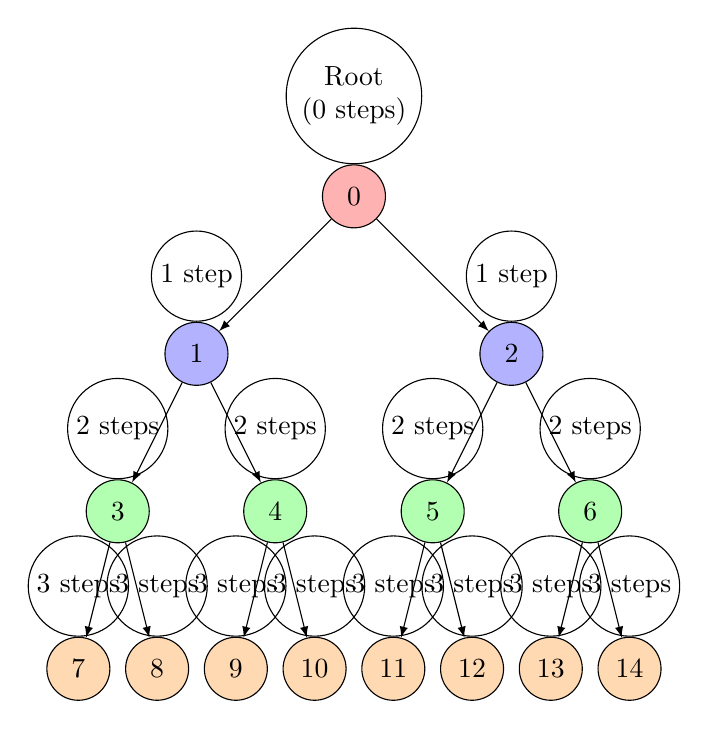
\begin{tikzpicture}[
    node distance=2cm,
    level 1/.style={sibling distance=4cm, level distance=2cm},
    level 2/.style={sibling distance=2cm},
    level 3/.style={sibling distance=1cm},
    every node/.style={circle, draw, minimum size=0.8cm, inner sep=2pt},
    edge from parent/.style={draw, -latex}
]
    % Root (Level 0)
    \node[fill=red!30] (0) at (0, 0) {0};
    
    % Level 1 nodes (k=1: labels 1, 2)
    \node[fill=blue!30] (1) at (-2, -2) {1};
    \node[fill=blue!30] (2) at (2, -2) {2};
    \draw[-latex] (0) -- (1);
    \draw[-latex] (0) -- (2);
    
    % Level 2 nodes (k=2: labels 3, 4, 5, 6)
    \node[fill=green!30] (3) at (-3, -4) {3};
    \node[fill=green!30] (4) at (-1, -4) {4};
    \node[fill=green!30] (5) at (1, -4) {5};
    \node[fill=green!30] (6) at (3, -4) {6};
    \draw[-latex] (1) -- (3);
    \draw[-latex] (1) -- (4);
    \draw[-latex] (2) -- (5);
    \draw[-latex] (2) -- (6);
    
    % Level 3 nodes (k=3: labels 7 to 14)
    \node[fill=orange!30] (7)  at (-3.5, -6) {7};
    \node[fill=orange!30] (8)  at (-2.5, -6) {8};
    \node[fill=orange!30] (9)  at (-1.5, -6) {9};
    \node[fill=orange!30] (10) at (-0.5, -6) {10};
    \node[fill=orange!30] (11) at (0.5, -6)  {11};
    \node[fill=orange!30] (12) at (1.5, -6)  {12};
    \node[fill=orange!30] (13) at (2.5, -6)  {13};
    \node[fill=orange!30] (14) at (3.5, -6)  {14};
    
    % Edges for Level 3
    \draw[-latex] (3) -- (7);
    \draw[-latex] (3) -- (8);
    \draw[-latex] (4) -- (9);
    \draw[-latex] (4) -- (10);
    \draw[-latex] (5) -- (11);
    \draw[-latex] (5) -- (12);
    \draw[-latex] (6) -- (13);
    \draw[-latex] (6) -- (14);
    
    % Annotations for step counts
    \node[align=center, above] at (0.north) {Root \\ (0 steps)};
    \node[align=center, above] at (1.north) {1 step};
    \node[align=center, above] at (2.north) {1 step};
    \node[align=center, above] at (3.north) {2 steps};
    \node[align=center, above] at (4.north) {2 steps};
    \node[align=center, above] at (5.north) {2 steps};
    \node[align=center, above] at (6.north) {2 steps};
    \foreach \n in {7,8,9,10,11,12,13,14} {
        \node[align=center, above] at (\n.north) {3 steps};
    }
\end{tikzpicture}
\end{document}